%!TEX root=../Mitschrift.tex
\clearpage
\section{Beschreibung der Aufgabe}
\subsection{Klassendiagramm}
	\begin{figure}[H]
	\centering
	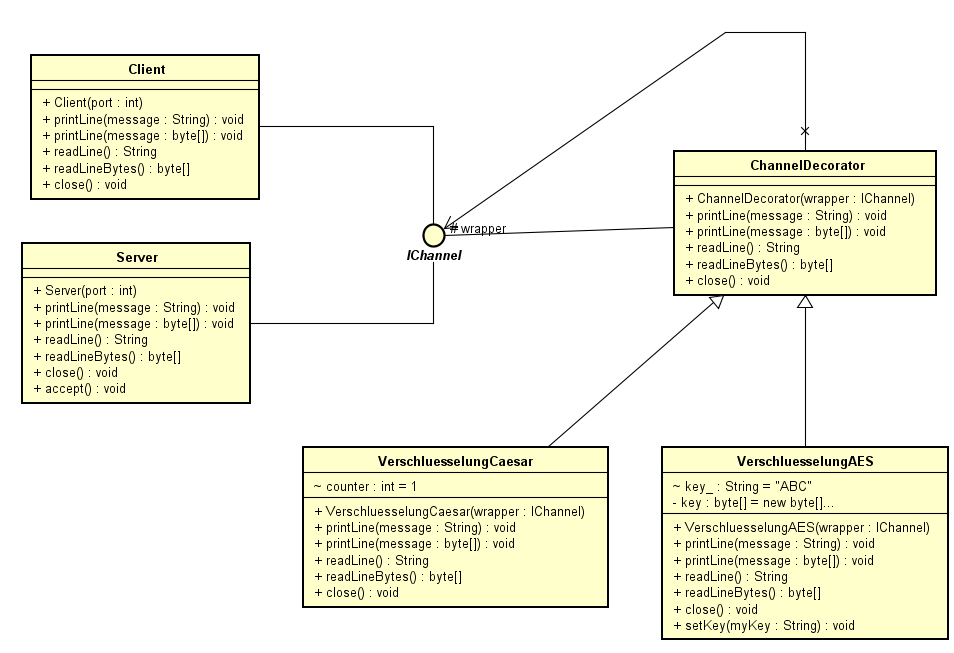
\includegraphics[width=1\textwidth]{images/abgabe.png}
	\caption{Klassendiagramm der Abgabe} 
\end{figure}
\subsection{Verbale Beschreibung}
Für die Aufgabe habe ich folgende Klassen erstellt:
\begin{itemize}
	\item \textit{Interface} \textbf{IChannel} :\\
		Es wurde das auf \href{https://elearning.tgm.ac.at/pluginfile.php/56383/mod\_assign/introattachment/0/IChannel.java?forcedownload=1}{moodle} zur Verfügung gestellte IChannel Interface verwendet. Dieses wird anschließend von allen Basisobjekten und dem Basisdecorator (\textbf{ChannelDecorator}) implementiert.
	\item Basisklasse \textbf{Server} implements Decorator:\\
		Im Server wird ein Serversocket erstellt und über dieses Socket mit dem Client kommuniziert. Dabei muss im Serversocket der Port angegeben werden über den die Kommunikation ablaufen soll.
	\item Basisklasse \textbf{Client} implements Decorator:\\
		Im Client wird ein Socket erstellt und über dieses Socket mit dem Server kommuniziert. Dabei muss im Socket die Adresse des Servers und der selben Port wie beim Server angegeben werden. (In unserem Fall wir das 'localhost' sein)
	\item Basisdecorator \textbf{ChannelDecorator} implements IChannel:\\14
		Der Basisdecorator ist die Basisklasse der Konkreten Decorator. Hier befindet sich der IChannel wrapper (''Der darüber liegende Decorator''). Außerdem wird in allen Methoden die selbige Methode des wrappers aufgerufen.
	\item ConcreteDecorator \textbf{VerschluesselungCaesar} extends ChannelDecorator:\\
		Der Konkrete Dekorator ''VerschluesselungCaesar''implementiert den Basisdecorator mit dem Verschlüsselungsalgorithmus ''Caesar''.
	\item ConcreteDecorator \textbf{VerschluesselungAES} extends ChannelDecorator:\\
	Der Konkrete Dekorator ''VerschluesselungAES''implementiert den Basisdecorator mit dem Verschlüsselungsalgorithmus ''AES''.
\end{itemize}
\section{Design Patterns}
\subsection{Wie können Design Patterns unterteilt werden}
Design Patterns werden prinzipiell in 3 Gruppen unterteilt:
\begin{enumerate}
	\item creational patterns
	\item structural patterns
	\item behavior patterns
\end{enumerate} 
\subsubsection{creational patterns}
creational (deutsch Erzeugungs-) Pattern werden bei der Erzeugung von Objekten verwendet. Hierbei wird die Erzeugung eines Objekts ausgelagert (meistens in eine eigene Klasse). Dadurch kann das Objekt entsprechend den Anforderungen erstellt werden.
Beispiele für Erzeugungs-Patterns:
\begin{itemize}
	\item Abstract Factory
	\item Builder
	\item Object Pool
	\item Prototype
	\item Singleton
\end{itemize}
\subsubsection{structural patterns}
structural (deutsch Strukturierungs-) Pattern regeln Beziehungen zwischen verschiedenen Klassen. Dadurch kann dann beispielsweise das Prinzip der Losen Koppelung eingehalten werden.
Beispiele für Strukturierungs-Patterns:
\begin{itemize}
	\item Decorator
	\item Proxy
	\item Adapter
	\item Flyweight
\end{itemize}
\subsubsection{behavior patterns}
Behavior (deutsch Verhaltens-) Pattern regeln die Kommunikation zwischen Objekten. 
  Beispiele für Verhaltens-Patterns:
  \begin{itemize}
  	\item Observer
  	\item Momento
  	\item Iterator
  	\item Interpreter
  \end{itemize}
\subsection{Wozu Design Patterns}
In der Softwareentwicklung gibt es gewisse Design-Prinzipien an die man sich halten sollte und die eine ''gute'' Software ausmachen. Diese sind:
\begin{itemize}
	\item Encapsulate what varies
	\item Favor composition over inheritance
	\item Program to interfaces, not implementations
	\item Strive for loosely coupled designs between objects that interact
	\item classes should be open for extentions but closed for modification 
	\item Depend on abstractions. Do not depend on concrete classes
\end{itemize}

Design Patterns helfen uns komplexere Probleme, bei denen eines oder mehrere dieser Prinzipien verletzt werden können, zu lösen und somit eine erweiterbare und flexible Software zu designen.
\clearpage 
\subsection{Übersicht existierender Design Patterns}
	\paragraph{Observer}~\\
Das Observer-pattern beschreibt wie ein Objekt welches in Beziehung mit vielen anderen Objekten steht , diese über Veränderungen benachrichtigt.
	\begin{figure}[H]
		\centering
		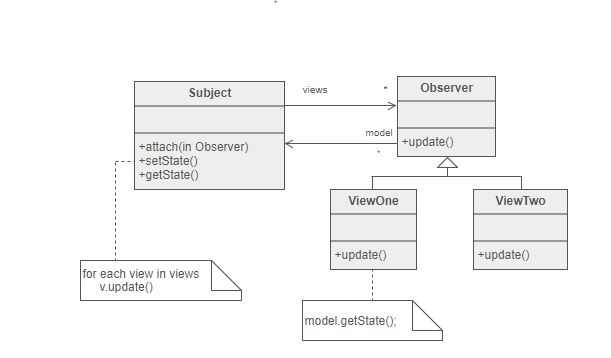
\includegraphics[width=0.5\textwidth]{images/Observer.png}
		\caption{Observer Pattern \\ $\href{https://sourcemaking.com/design_patterns/observer}{https://sourcemaking.com/design_patterns}$}
	\end{figure}
	\paragraph{Decorator}~\\
Das Decorator-Pattern ist ein \textbf{structural pattern}. Erlaubt Veränderungen der Eigenschaften eines Objekts während der Laufzeit
	\begin{figure}[H]
		\centering
		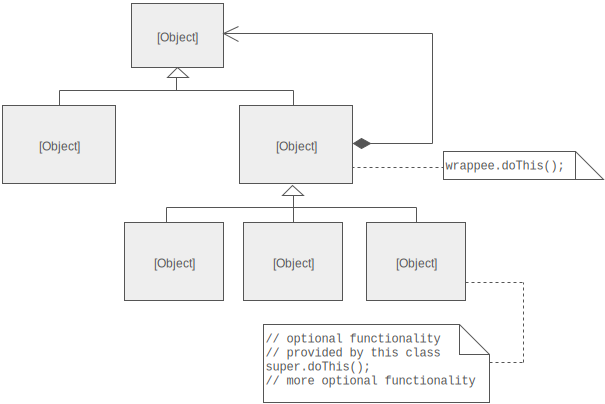
\includegraphics[width=0.5\textwidth]{images/Decorator.png}
		\caption{ Descorator Pattern \\ $\href{https://sourcemaking.com/design_patterns/decorator}{https://sourcemaking.com/design_patterns}$}
	\end{figure}
	\paragraph{Factory}~\\
Das Factory-Pattern ist ein \textbf{Creational pattern}. Hierbei wird ein Objekt in einer ''Factory'' erstellt ohne, dass der Client weiß wie dieses erstellt wurde. Man kennt lediglich das Interface des Objekts , weiß jedoch nicht wie die Konkrete Implementation aussieht.
\begin{figure}[H]
	\centering
	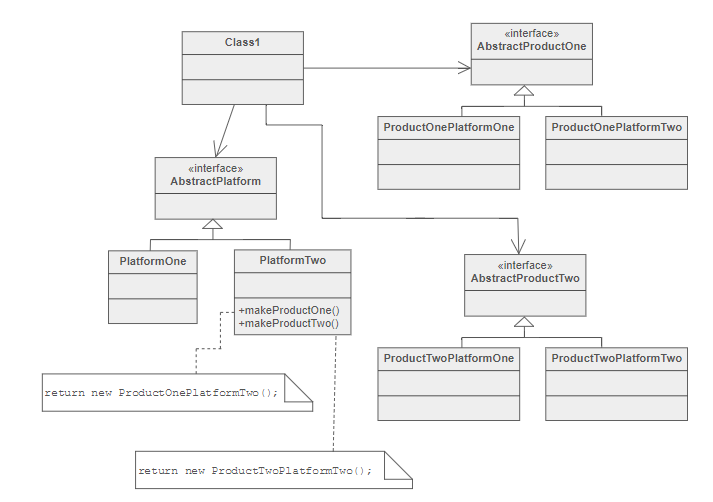
\includegraphics[width=0.5\textwidth]{images/Factory.png}
	\caption{Factory Pattern \\ $\href{https://sourcemaking.com/design_patterns/factory}{https://sourcemaking.com/design_patterns}$}
\end{figure}
	\paragraph{Strategy}~\\
Das Strategy-Pattern ist ein \textbf{Behavioral pattern}. Hierbei werden zu einer Aufgabe mehrere austauschbare ''Strategien'' in Form von verschiedenen Algorithmen zur Verfügung gestellt. 
\begin{figure}[H]
	\centering
	\includegraphics[width=0.5\textwidth]{images/strategy.png}
	\caption{Strategy Pattern \\ $\href{https://sourcemaking.com/design_patterns/strategy}{https://sourcemaking.com/design_patterns}$}
\end{figure}
\clearpage
\section{Decorator Pattern}
	\subsection{Allgemeines Klassendiagramm}
\begin{figure}[H]
	\centering
	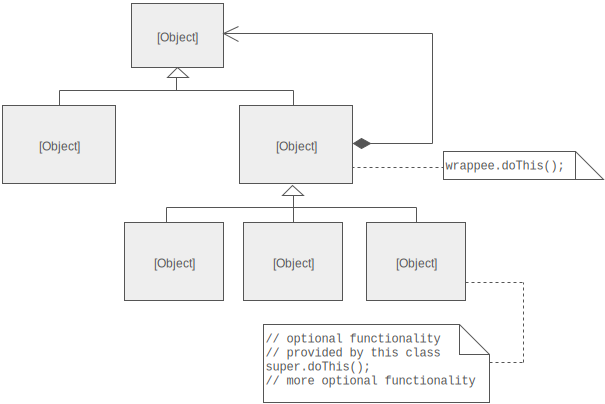
\includegraphics[width=1\textwidth]{images/Decorator.png}
	\caption{ Descorator Pattern \\ $\href{https://sourcemaking.com/design_patterns/decorator}{https://sourcemaking.com/design_patterns}$}
\end{figure}
	\subsection{Grundzüge des Design Patterns}
Das Decorator Pattern wird dann verwendet, wenn eine Instanz eine Klasse mit weiteren Instanzen dieser Klasse erweitert werden soll.
	\subsection{Vor- und Nachteile}
\begin{itemize}
	\item \textbf{Flexibilität} \\ 
 Es können Objekte einer Klasse um Objekte der selben Klasse erweitert werden und so das Verhalten von Objekten zur Laufzeit modifiziert werden.
	 \item \textbf{Erweiterbarkeit}\\
 Das Programm ist geschlossen für Veränderungen und offen für Erweiterungen. Es können immer wieder neue Objekte zu unserer Software erstellt werden mit dem andere erweitert werden können.
	 \item \textbf{Nicht Redundant}\\
 Im Vergleich zur Vererbung wird Coderedundanz vermieden. Es wird ein jedes Verhalten nur ein mal implementiert. $\rightarrow$ Fehlervermeidung
\end{itemize}

	\subsection{Weitere Anwendungsfälle}
\begin{itemize}
	\item \textbf{Erweiterung von Objekten}\\
	Immer dann wenn in einem Objekt mehrere Gleichartige Funktionen angehängt werden sollen wie z.B. in unserem Verschlüsselungsbeispiel , hier sollen mehrere Verschlüsselungsarten auf einen Text dynamisch angewendet werden.
	\item \textbf{Funktionalitätsänderungen während der Laufzeit}\\
	Wenn die Software darauf ausgelegt sein soll in der Laufzeit Funktionalitäten hinzuzufügen oder Entfernen zu können
	\item \textbf{Unabhängigen Erweiterungen}\\
	Wenn Erweiterungen unabhängig voneinander sind wird es unpraktisch Vererbung dafür zu benutzen. Hierfür empfiehlt es sich eher auf den Decorator zurückzugreifen.
	
\end{itemize}

\clearpage
\section{Strategy Pattern}
\subsection{Allgemeines Klassendiagramm}
\begin{figure}[H]
	\centering
	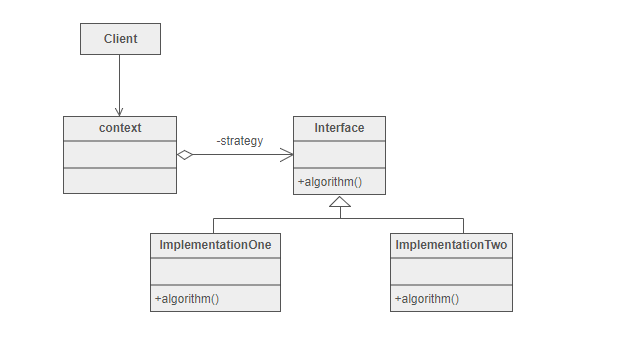
\includegraphics[width=1\textwidth]{images/Strategy.png}
	\caption{ Descorator Pattern \\ $\href{https://sourcemaking.com/design_patterns/strategy}{https://sourcemaking.com/design_patterns}$}
\end{figure}
\subsection{Grundzüge des Design Patterns}
Das Strategy Pattern wird verwendet wenn ein Objekt mehrere Arten sich in bestimmten Situationen zu verhalten. Diese Verhaltensarten können auch in der Laufzeit geändert werden. 
\subsection{Vor- und Nachteile}
\begin{itemize}
	\item \textbf{Vermeidung von Vererbung} \\ 
	In Programmiersprachen ohne Mehrfach-Vererbung entnimmt man dadurch nicht die ''super Klasse''. Es können Immer neue Verhaltensarten zur laufzeit hinzugefügt werden ohne Codeänderungen in der ''Basisklasse''. 
	\item \textbf{Wiederverwendbarkeit}\\
	Da die Verhaltens-Klassen abstrakt sind kann diese unabhängig von der Basisklasse verwendet wird. $\rightarrow$ Entkoppelung
	\item \textbf{''Composition over inharitance''}\\
	Müssten mehrere Verhaltensarten gleichzeitig in der ''Basisklasse'' implementiert werden würde dies nach einigen implementierten Verhalten schnell zu ''Spaghetticode'' führen durch die vielen \textit{if-else} statements die hierfür benötigt werden würden. 
	\item \textbf{prototypen}\\
	Vorallem bei Prototypen bei denen man sich noch unsicher über den letztendlichen Algorithmus ist oder wo noch Performance optimierte Algorithmen zu einem späteren Zeitpunkt implementiert werden empfiehlt es sich diese nicht ''Fest verwurzelt'' in der Programmlogik zu haben. 
\end{itemize}



\subsection{Weitere Anwendungsfälle}
\begin{itemize}
	\item \textbf{Klassen die sich nur im Verhalten unterscheiden}\\
	Wenn mehrere Klassen die sich komplett bis auf ein Verhalten ähneln erstellt wurden ist das ein gutes Zeichen dafür dass hierbei die Verwendung des Strategy Patterns von Vorteil wäre.
	
	\item \textbf{Unabhängigen Erweiterungen}\\
	Wenn Erweiterungen unabhängig voneinander sind wird es unpraktisch Vererbung dafür zu benutzen. Hierfür empfiehlt es sich eher auf den Decorator zurückzugreifen.
	
\end{itemize}

\clearpage
\section{resources}
https://sourcemaking.com/design\_patterns
https://refactoring.guru/design-patterns/creational-patterns
https://www.philipphauer.de/study/se/design-pattern/decorator.php
